\RequirePackage{docswitch}
\setjournal{\flag}

\documentclass[\docopts]{\docclass}


\usepackage{lsstdesc_macros}

\usepackage{graphicx}
\graphicspath{{./}{./figures/}{.logos}}
\bibliographystyle{apj}


\newcommand{\textul}{\underline}
\newcommand{\qp}{\texttt{qp}}
\newcommand{\pz}{photo-$z$ PDF}
\newcommand{\Pz}{Photo-$z$ PDF}


\begin{document}

\title{ Approximating photo-z PDFs for large surveys }


\begin{abstract}

Upcoming and ongoing galaxy surveys will produce redshift probability 
distribution functions (PDFs) in addition to traditional photometric redshift 
(photo-$z$) point estimates.  However, the storage of \pz s may present a 
challenge with increasingly large catalogs, as we face a trade-off between the 
accuracy of subsequent science measurements and the storage cost.  This paper 
presents \qp, a Python package facilitating manipulation of approximations of 
1-dimensional PDFs, as suitable for \pz s.  We use \qp\ to investigate the 
performance of three PDF formats on two realistic datasets representative of 
upcoming surveys with different data qualities as a function of the number of 
stored parameters per \pz, using metrics of both individual \pz s and an 
estimator of the overall redshift distribution function.

\end{abstract}

\dockeys{methods: data analysis, catalogs, surveys}

\maketitlepost





\section{Introduction}
\label{sec:intro}


Ongoing and upcoming photometric galaxy surveys such as the Large Synoptic 
Survey Telescope (LSST) will observe tens of billions of galaxies without 
spectroscopic follow-up to obtain redshifts necessary for studies of cosmology 
and galaxy evolution, instead relying on the methods of photometric redshift 
(photo-$z$) estimation.  Photo-$z$s are subject to a number of systematic 
errors, some caused by the data analysis procedures and others intrinsic to the 
data itself.  Due to these issues, the photo-$z$ community has come to favor 
estimation of redshift probability distribution functions (PDFs), or \pz s, 
that include information about the potential for such systematic errors for 
each galaxy in the survey.  \Pz s are interim posterior distributions, as they 
are estimates of the probability of a galaxy's redshift conditioned on its 
photometric data and any assumptions made by the method producing it, though 
they are commonly written simply as $p(z)$.

Given the tremendous size of the surveys in question, storage of these 
probability distributions involves making difficult decisions.  Each survey 
seeks to create a catalog of \pz s balancing accuracy against storage 
footprint.  For example, the \pz\ catalog that LSST will release is limited to 
200 floating point numbers per galaxy, with plans to store \pz s derived by 
multiple methods.  \citep{juric_data_2017}
These matters were first addressed in \citet{carrasco_kind_sparse_2014} in the 
context of a single galaxy survey, a limited set of storage formats, and 
metrics restricted to that survey's intended \pz\ use case.  The number of 
stored parameters and the parametrization optimizing this choice, however, 
depend on the science requirements of the survey and the characteristics of the 
data.  This paper answers the question of \textit{how} these choices should be 
made in general, demonstrating the approach on diverse mock data and using 
mathematically motivated metrics of both the individual \pz s and a science 
application.  The publicly available \qp\ Python package is also presented here 
as a tool to enable each survey to optimize these choices.

In Sec. \ref{sec:methods}, we outline how \qp\ can be used to optimize the 
choice of storage format and catalog allocation.  In Sec. \ref{sec:data}, we 
describe the mock datasets on which we perform such an analysis.  We present 
the results of this procedure in Sec. \ref{sec:results} and make 
recommendations for the use of \qp\ by the photo-$z$ community in 
\ref{sec:conclusions}.








\section{Methods}
\label{sec:methods}



We have developed the \qp\ Python package to facilitate manipulation of \pz s.  
A \texttt{qp.PDF} object is defined by its parametrizations.  By way of 
interpolation, \qp\ can convert a representation of a \pz\ under one 
parametrization to a representation of that \pz\ under a different 
parametrization.  The currently supported parametrizations are described in 
Sec. \ref{sec:approx}.  \qp\ also includes a few built-in metrics of the 
accuracy of a representation of a \pz\ if its value under a given 
parametrization is designated as "true."  The currently implemented metrics are 
described in Sec. \ref{sec:metric}.

\subsection{Approximation Methods}
\label{sec:approx}



First, we establish a vocabulary for the definitions of approximation methods.  
Each \textit{parametrization} of a \pz\ is defined in terms of the 
\textit{format} function $\mathcal{F}$, \textit{metaparameters} comprising 
$\vec{C}$, and \textit{parameters} comprising $\vec{c}$.  Each parametrization 
in turn corresponds to a \textit{representation}
\begin{align}
  \label{eq:definition}
  \hat{p}_{\mathcal{F}, \vec{C}, \vec{c}}(z) &\equiv \mathcal{F}_{\vec{C}}(z | 
\vec{c})
\end{align}
of the \pz, denoted as $\hat{p}(z)$ for brevity.  We often employ interpolation 
schemes with a generic interpolator functions $F_{\vec{C}'}(z; z', p')$ that 
comes with its own $N_{M}'$ metaparameters $\vec{C}'$.  The choice of 
interpolator may be made on a survey-by-survey basis.  \qp\ supports all 
interpolation options available to the \texttt{scipy.interpolate.interp1d} 
function.  However, we have chosen a default interpolation scheme for each 
format to maximize its performance, demonstrating the significance of the 
choices made in reconstructing a \pz\ from stored parameters.

\qp\ is currently capable of converting a \pz\ between five formats that are 
described below in terms of the number $N_{f}$ of stored parameters $c_{i}$ per 
\pz, which are presumed to be floating point numbers unless otherwise 
specified.  The metaparameters are a set of $N_{M}$ numbers $C_{i}$ necessary 
to convert the stored \pz\ parameters $\vec{c}$ into a probability distribution 
function over redshift.  Because the metaparameters for a catalog of \pz s 
released by a survey will only need to be stored once, it does not matter how 
large $N_{M}$ is.

Three of these formats are considered candidates for large survey \pz\ catalog 
storage: regular binning (Sec. \ref{sec:bins}), random samples (Sec. 
\ref{sec:samples}), and regular quantiles (Sec. \ref{sec:quantiles}), while the 
other two, regular evaluations (Sec. \ref{sec:grid}) and mixture models (Sec. 
\ref{sec:mm}), are used solely for internal manipulations within \qp, but are 
nonetheless discussed here for completeness.  The different formats are 
illustrated in Fig. \ref{fig:qp} on a multimodal \pz\ with stored parameters.  
For each format, we address the following questions:

\begin{itemize}
  \item When/where has this format appeared in the literature as a published 
catalog format, native \pz\ code output format, and science application input 
format?
  \item What exactly is stored under this format, per galaxy (the parameters) 
and per catalog (the metaparameters)?
  \item Beyond fidelity to the original \pz, what are the a priori strengths 
and weaknesses of this format, especially with respect to 
compression/reconstruction properties?
\end{itemize}

\begin{figure}
  \includegraphics[width=0.9\columnwidth]{figures/Euclid_example_pz.png}
  \caption{\qp\ can approximate a continuous 1D PDF (black line) using the step 
function (red dashed), random sample (green short-dashed), and quantile formats 
(blue long-dashed) with a specified number of stored parameters (20 in this 
case).
  \label{fig:qp}}
\end{figure}

\subsubsection{Regular Binning}
\label{sec:bins}

By far the most popular format for \pz s is that of a piecewise constant step 
function, also called a histogram binning.  The only format that has been used 
for public release of \pz\ catalogs \citep{tanaka_photometric_2017, 
sheldon_photometric_2012}; it is unclear whether this is a consequence or a 
cause of the fact that it is the most common format for using \pz s in 
cosmological inference, as tomographic binning is a universal step between the 
\pz\ catalog and calculation of any two-point correlation function.

The metaparameters of the binned parametrization are the ordered list of 
$N_{M}=N_{f}+1$ redshifts $\vec{C} = (z_{1}, z_{2}, \dots, z_{N_{M}-1}, 
z_{N_{M}})$ with $C_{1} < C_{2} < \dots < C_{N_{M}-1} < C_{N_{M}}$ serving as 
endpoints shared by all galaxies in the catalog, each adjacent pair of which is 
associated with a parameter $c_{i}=\int_{C_{i}}^{C_{i+1}}\ p(z)dz$.  The format 
function $\mathcal{F}^{b}=\sum_{i=1}^{N_{f}}F_{i}$ is the sum of a set of 
$N_{f}$ step functions $F_{i}$, where a step function is defined as
\begin{align}
  \label{eq:step}
  F_{C_{i}, C_{i+1}}(z| (C_{i}, C_{i+1})), c_{i}) &= c_{i} 
\left\{\begin{tabular}{cc}$1$&$C_{i}<z<C_{i+1}$\\
0&$z < C_{i}$\ or\ $z > C_{i+1}$\end{tabular}\right\},
\end{align}
making the estimator of the \pz\
\begin{align}
  \label{eq:binned}
  \hat{p}_{b}(z) &= \sum_{i}^{N_{f}}\ c_{i} 
\left\{\begin{tabular}{cc}$1$&$C_{i}<z<C_{i+1}$\\
0&$z < C_{i}$\ or\ $z > C_{i+1}$\end{tabular}\right\}
\end{align}
under the binned format.  We note that a step function may be considered an 
interpolator that is uniform between given endpoints.

If the binning is "regular," then $C_{i+1}=C_{i}+\Delta$ for some constant 
scalar $\Delta$.  As this is the only type of binning that has been used in the 
literature, it is the only one we consider.  (A suitable irregular binning 
across the entire catalog would also require a nontrivial optimization.)  The 
standard assumption that $p(z)=0$ when $z<C_{1}$ or $z>C_{N_{M}}$ implies that 
the $c_{i}$ are normalized according to $\sum_{i} c_{i}\cdot\Delta = 1$.  Note 
that this is not equivalent to the erroneous normalization condition $\sum_{i} 
c_{i} = 1$ that commonly appears in the literature.

All known native \pz\ formats are easy to convert to the histogram 
representation.  However, the corrolary to this statement is that it is an 
inherently lossy format.  A histogram parametrization with bin widths larger 
than features of the \pz\ may not accurately represent the underlying 
probability distribution, as significant structure may be lumped into a single 
bin value.  This problem may be particularly troubling as the quality of the 
approximation may not be unbiased among catalog entries; rather, it is likely 
to correlate with the properties of the \pz\ in question and thus the true 
redshift of the galaxy.

The binned parametrization may also be considered wasteful in terms of data 
storage.  A \pz\ with a compact probability distribution, with much of the 
probability contained within a region far narrower than the redshift range 
$z_{N_{M}} - z_{1}$, may have many of its catalog entries $c_{i}$ being 
identically zero.  The storage footprint of this data is wasted in that it is 
redundant, with each $c_{i}$ requiring the same space even though 
$c_{i}=c_{i'}$ for many pairs $(i, i')$.  (A similar case can be made for a 
very flat distribution, where all $c_{i}$ are approximately the same.)

Finally, the binned parametrization requires the researcher to choose the 
minimum and maximum possible redshifts of the galaxy sample.  These are 
physical quantities that are unknown, so it would be preferable to not have to 
choose them at the stage of producing the \pz\ catalog.

\subsubsection{Random Samples}
\label{sec:samples}

Samples are the native output format of many machine learning algorithms 
dependent on random choices, such as random forests.
Such approaches typically produce large numbers of samples, far more than can 
realistically be stored by any survey, so a subsample is commonly stored.

The parameters of the samples format are the set of samples $\vec{c}=(z_{1}, 
z_{2}, \dots, z_{C_{0}-1}, z_{C_{0}})$.  An implicit metaparameter is simply 
$C_{0}=N_{f}$, meaning $N_{M}=1$.  Though it is possible to construct a catalog 
where each galaxy has a different number $N_{f}$ of stored samples (and thus a 
different value of $C$), optimizing the choice of $N_{f}$ given the shape of 
the \pz\ in its native format is nontrivial.  As this has not been done in the 
literature, we leave its investigation to future work.  To reconstruct the 
probability distribution, the format function $\mathcal{F}^{s}$ is the 
interpolation scheme $F$, such as a kernel density estimate (KDE), operating on 
another function $\Phi(z)=p$, such as a KDE's kernel function, that transforms 
samples into probability density estimates, which also has metaparameters 
$\vec{C}''$ such as a smoothing bandwidth of the kernel function.  The samples 
representation is then
\begin{align}
  \label{eq:sampled}
  \hat{p}_{s}(z) &= F_{\vec{C}'}(z | \vec{c}, \Phi_{\vec{C}''}(\vec{c})).
\end{align}

As with the histogram format, it is in general easy to convert any format into 
samples, at the risk of loss of information.  One risk of samples is that a 
small number of samples from a broad \pz\ may not be representative of the 
overall shape, boosting the variance across the catalog.  On the other hand, a 
small number of samples can be a very efficient way to store \pz s with narrow 
features.  As in the case of the histogram parametrization, the quality of the 
approximation may be correlated to properties of the \pz\ that themselves 
correlate with redshift.  Unlike the simple reconstruction scheme for the 
histogram format (Eq. \ref{eq:binned}), there is no straightforward 
interpolation for samples.  When we need one for the purposes of calculating 
metrics, we use a kernel density estimate, which may introduce additional loss 
of information, with the degree of that imprecision depending on nuisance 
parameters of the interpolation scheme, i.e. the smoothing kernel and bandwidth.

\subsubsection{Regular Quantiles}
\label{sec:quantiles}

One parametrization that has not previously been implemented is that of 
quantiles, which are defined in terms of the cumulative distribution function 
(CDF)
\begin{align}
  \label{eq:cdf}
  CDF(z) &= \int_{-\infty}^{z}\ p(z')\ dz'.
\end{align}
Under the quantile format, an ensemble of \pz s shares a set of $N_{M}=N_{f}$ 
values $\vec{C}=(q_{1}, q_{2}, \dots, q_{N_{f}-1}, q_{N_{f}})$ with 
$0<q_{1}<q_{2}<\dots<q_{N_{f}-1}<q_{N_{f}}<1$.  Each galaxy's catalog entry is 
the vector of redshifts $\vec{c}=(z_{1}, z_{2}, \dots, z_{N_{f}-1}, z_{N_{f}})$ 
satisfying $CDF(c_{i})=C_{i}$, so the quantile format function 
$\mathcal{F}_{q}$ is the derivative of an interpolation of the inverse CDF 
$CDF^{-1}(C_{i})=c_{i}$ under the interpolation scheme $F$.  The format 
function is then the convolution $\mathcal{F}^{q}=F(CDF^{-1})$, making the 
quantile representation
\begin{align}
  \label{eq:quantiles}
  \hat{p}_{q}(z) &= F_{\vec{C}'}(z| \vec{c}, \frac{d}{dz}CDF^{-1}(\vec{C})).
\end{align}
In our tests, the quantiles are regular, such that $C_{i}\equiv i\bar{C}$, 
where $\bar{C}\equiv(N_{f}+1)^{-1}$, but \qp\ does not require that this be so. 
 Additionally, in the tests presented here, we use a linear interpolator by 
default for the quantile format.

As no survey has previously stored quantile \pz s, no existing \pz\ code 
produces quantiles as output, and no science case pipeline has yet been 
developed to accept input \pz s in the quantile format.  Given its limited 
visibility, we share why it is the subject of this study.  The quantile 
parametrization is the inspiration for this work and namesake of \qp.  Though 
it has not appeared in the \pz\ literature prior to this point, it is a natural 
choice for the compression of probability distributions because it keeps more 
information in areas of higher probability density, so there is inherently less 
waste in the information that is stored for each catalog entry and minimal risk 
of bias in the quality of the approximation across \pz\ shapes.  Storing 
quantiles is equivalent to storing piecewise constant data on an irregular 
binning optimized to have narrower bins in areas of high probability and wider 
bins in areas of low probability, effectively performing the optimization in 
bin size while still permitting an entire catalog to share a single set of 
metaparameters.  Unlike samples, its performance is uncorrelated with the shape 
of the \pz.

Though the strengths and weaknesses of quantiles have not yet been formally 
explored, we know have some ideas of what may be at play.  One obvious issue is 
that storing more information where there is more probability density may not 
always be desirable; it is possible that for some applications, information 
about the tails of the \pz, where $z<c_{1}$ or $z>c_{N_{f}}$, is valuable.  
This may be mitigated somewhat if endpoints are chosen, as is already done for 
the histogram format.  Unlike thebounding bins of the histogram format, the 
quantile format still has substantial freedom if the endpoints are informed by 
a broad prior (i.e. we have no qualms about demanding $0<z<10$).  As with the 
samples representation, an interpolation function must be chosen for 
reconstructing the \pz\ from the stored parameters.  Some native \pz\ output 
formats, like samples, are easy to convert to regular quantiles, while others, 
like piecewise constant functions, are not, requiring a numerical optimization 
for each stored parameter $c_{i}$.

\subsubsection{Regular Evaluations}
\label{sec:grid}

A common format that appears in the \pz\ literature is that of evaluations of 
the probability at specified points.  In particular, it is the most popular 
native format for \pz s produced by template-fitting codes like BPZ.  
\citep{benitez_bayesian_2000}  The reason for this is that with a large SED 
template library, it is more efficient to precompute the colors of an SED at a 
particular redshift than to do it on the fly while fitting the SED and redshift 
of an individual galaxy's photometry.  The native parametrization of BPZ, for 
example, has many more parameters than can reasonably be stored, so we do not 
consider this format in this study.  We do, however, use it for internal 
manipulations when converting between formats and for the evaluation of 
metrics, so we describe it in the same notation as the other formats discussed.

The format of grid evaluations has stored parameters $\vec{c}=(p(z_{1}), 
p(z_{2}), \dots, p(z_{N_{f}-1}, p(z_{N_{f}}))$ on a grid of $N_{M}=N_{f}$ 
redshifts $\vec{C}=(z_{1}, z_{2}, \dots, z_{N_{M}-1}, z_{N_{M}})$ serving as 
metaparameters.  To reconstruct the \pz\ from the stored parameters using the 
format function $\mathcal{F}^{g}$, one must again choose an interpolation 
scheme $F$.  The reconstruction can then be written as
\begin{align}
  \label{eq:gridded}
  \hat{p}_{g}(z) &= F(z| \vec{C}, \vec{c}).
\end{align}
It has thus far only been applied on a regular grid in redshift (i.e. 
$\Delta=C_{i+1}-C_{i}$ for a constant $\Delta$) shared among the entire 
catalog.  As irregular grids have not been used in the literature, we do not 
consider them nor grids that are not homogeneous over the catalog, though \qp\ 
can accommodate them.  We use a linear interpolator in the tests presented in 
this study.

The gridded parametrization is in some ways similar to the histogram format of 
\ref{sec:bins}, suffering from the same risks of losing small-scale features 
(and the corresponding risk of systematics in the quality of the approximation) 
when the resolution is too low, wasting a substantial fraction of the $N_{f}$ 
allocated parameters if the distribution is compact, and having to choose the 
grid endpoints for the ends of the distribution.  Like the piecewise constant 
parametrization, the grid evaluations may need to be normalized before they can 
be used as a mathematically valid \pz.

\subsubsection{Mixture Model}
\label{sec:mm}

There is some history of using a mixture model parametrization for \pz s, 
particularly that of a small number of Gaussian components.
A Gaussian mixture model may be a natural choice for the native output of a 
method based on a distance metric in the space of photometry because the \pz s 
could be weighted sums of Gaussians by construction, though for many other 
methods, there is no such guarantee.  Besides the mixture of Gaussians, other 
functions have been investigated before in the sparse basis representation of 
\citet{carrasco_kind_sparse_2014}, which uses a mixture model of members of a 
library of $N_{M}\sim10^{4}$ functions.

Under the mixture model format, the format function $\mathcal{F}^{m}$ is a 
weighted sum of $N_{M}'$ continuous functions $\phi^{j}(z)$ chosen from a set 
of $N_{M}''$ possible functions, each with $N_{M}^{j}$ metaparameters in 
$\vec{C}^{j}$ and $N_{f}^{j}$ parameters unique to each galaxy.  Because each 
component need not have the same $N_{M}^{j}$, the number of possible components 
for a fixed $N_{f}$ is not constrained.  Because $N_{M}^{j}$ is not necessarily 
the same for all model components $j$, a single $N_{f}$ is not necessarily 
something that reasonably can be imposed on the catalog if the functional forms 
are not specified, and even if they are, there is no easy way to require that 
$\sum_{j=1}^{N_{M}'}N_{M}^{j}=N_{f}$ if $N_{f}$ is fixed.  Each component 
function would have at least one metaparameter $C_{0}^{j}$ to identify the 
functional form of $\phi^{j}$, corresponding to $c_{0}^{j}=C_{0}^{j}$.  If 
$\phi^{j}(z)$ is a function with $N_{M}^{j}$ total parameters, any subset of 
them may be fixed over the catalog and designated as components of 
$\vec{C}^{j}$ or left free to be unique for each galaxy, making the remainer 
components of $\vec{c}^{j}$.

To keep these tests simple, we make three assumptions: (1) there are no 
metaparameters $\vec{C}_{j}$ of the component functions $\vec{\phi}_{j}(z)$ 
that are fixed over the catalog, (2) all component functions 
$\vec{\phi}_{j}(z)$ are probability distribution functions that are positive 
semidefinite and integrate to unity, and (3) all component probability 
distribution functions $\phi_{j}(z)$ are Gaussian probability distribution 
functions $\mathcal{N}(z | 
\mu_{j},\sigma^{2}_{j})\equiv(2\pi\sigma^{2})^{-1/2}\exp[-(z-\mu)^{2}/2\sigma^{2
}]$.  (2) is a requirement we actively impose in \qp\ so that even a mixture 
model with a single component is a valid representation of a \pz.  Together, 
(1) and (2) also imply that we can designate $c_{0}^{j}=w_{j}$ as a weight 
coefficient for the $j^{th}$ component of a galaxy's \pz, where 
$\sum_{j=1}^{N_{M}'}w_{j}=1$.  Knowing that each Gaussian component is 
specified by the $N_{M}^{j}=3$ parameters of weight $w_{j}$, mean $\mu_{j}$, 
and variance $\sigma^{2}_{j}$, (3) permits us to constrain $N_{M}'\leq 
N_{f}/3$.  Under these assumptions, the representation $\mathcal{F}^{m}$ is
\begin{align}
  \label{eq:gmm}
  \hat{p}_{m}(z) &= \sum_{j=1}^{N_{M'}} c_{0}^{j} \mathcal{N}(c_{1}^{j}, 
c_{2}^{j}),
\end{align}
subject to the normalization of the weights mentioned above.

In this work, the common Gaussian mixture model of Eq. \ref{eq:gmm} is the only 
one we consider, though the \qp\ framework can accommodate mixtures of all 
probability distribution functions implemented as 
\texttt{scipy.stats.rv\_continous} objects.  Besides the mixture of Gaussians, 
other functions have been investigated before in the sparse basis 
representation of \citet{carrasco_kind_sparse_2014}, which uses a mixture model 
of members of a library of $N_{M}'\sim10^{4}$ functions with metaparameters 
$\vec{C}$ that are identification numbers for each function in the library; 
$\vec{c}$ under this parametrization is just an array of the identification 
numbers of the $N_{f}$ library functions whose sum best approximates the 
original \pz.

Though it has promising compression properties, we do not consider the sparse 
basis format in this work for several reasons.  Decomposition with 
\texttt{SparsePZ} does not enforce that the stored parametrization be a 
probability distribution in the mathematical sense of integrating to unity and, 
especially, always being positive semidefinite.  While normalizing a positive 
semidefinite function to integrate to unity is always possible (if the 
endpoints of integration are specified), one can motivate multiple schemes for 
enforcing nonnegativity that result in different reconstructions $\hat{p}(z)$.  
To discourage misuse of \qp, we do not permit functions that can take negative 
values at this time.
We anticipate including the sparse basis representation in \qp\ in future work 
when we can justify a choice of how to handle negative values.


Mixture models can be stored with very few parameters per component function 
and are trivial to convert to piecewise constant functions, samples, and 
evaluations commonly used for analysis.  Compressing an original \pz\ into this 
format may be difficult due to necessity of an optimization, such as a 
least-squares fit.  However, that challenge is balanced by the ease of 
reconstructing an estimated $\hat{p}(z)$ from its stored parameters, as no 
interpolation is even necessary.  A mixture model, however, is only an accurate 
approximation of a \pz\ \textit{if they are actually comprised of the included 
functions}.  If, for example, the \pz\ is not inherently a sum of Gaussian 
components, it could take a prohibitive number of Gaussian components to obtain 
an acceptable approximation.  Because the mock data discussed here is not known 
to be comprised of a weighted sum of Gaussian components, we do not test the 
mixture model against other formats.

\subsection{Comparison Metrics}
\label{sec:metric}


In contrast to popular \pz\ metrics in the literature, we aim to probe how 
closely a PDF $\hat{p}(z)$ reconstructed from a limited set of parameters 
approximates a true PDF $p(z)$, so there is no notion of the accuracy of either 
the approximate nor the original \pz\ relative to a galaxy's true redshift.  
For a demonstration of how one might approach the different problem of 
evaluating the accuracy of a \pz\ relative to a true redshift, see Schmidt, et 
al. (in prep.).)  To quantify how much more information is in a true PDF $P(z)$ 
than an approximate PDF $P'(z)$, we use the Kullback-Leibler divergence (KLD), 
defined as
\begin{align}
  \label{eq:kld}
  KLD[P(z) || P'(z)] &= \int_{-\infty}^{\infty}\ P(z)\ 
\log\left[\frac{P(z)}{P'(z)}\right]\ dz
\end{align}
Though the KLD is hardly unheard of in astronomy, it is far from established.  
In App. \ref{sec:kld}, we review its properties and deepen intuition, as it is 
central to the proposed procedure for choosing the best storage parametrization 
for \pz\ catalogs.

The most important quirk of the KLD is its asymmetry; it is not a distance, 
like the root mean square error, that is the same from $P(z)$ to $P'(z)$ as it 
is from $P'(z)$ to $P(z)$ but a \textit{divergence} in the information lost 
when using $P'(z)$ to approximate $P(z)$.  The KLD requires not only that both 
functions $P(z)$ and $P'(z)$ be true probability distributions but also that 
there must be some notion of a true reference distribution.  The former 
condition is not always satisfied for the binned, gridded, and mixture model 
formats produced by \pz\ code so must be explicitly enforced.  The latter is in 
general not true for real data but can be checked for mock data.  It is also 
obvious that the KLD is always positive, and a smaller value indicates better 
agreement between the approximation and the truth.

\Pz s have thus far been used almost exclusively to estimate the redshift 
distribution function $n(z)$ necessary for calculating the correlation 
functions used by many cosmological probes.  The most common way to estimate 
the redshift distribution function is to sum the \pz s according to
\begin{align}
  \label{eq:nz}
  \hat{n}(z) &\equiv \frac{1}{N_{g}}\ \sum_{k=1}^{N_{g}}\ \hat{p}^{k}(z),
\end{align}
in terms of the number $N_{g}$ of galaxies $k$ in the catalog, where the 
estimator is normalized so that it, too, is a probability distribution (though 
in the literature it is often subject to the fallacy conflating a sum and an 
integral, first mentioned in Sec. \ref{sec:bins}).  We do not recommend this 
approach to estimating the redshift distribution (see Malz and Hogg, et al. (in 
prep.) for a mathematically consistent alternative), however, we use it under 
the assumption that any metric calculated on a more principled estimator of the 
redshift distribution function will have similar behavior with respect to the 
parametrization of the \pz\ catalog as that of the stacked estimator.

As $n(z)$ is itself a PDF (though in the literature it is often subject to the 
fallacy conflating a sum and an integral, first mentioned in Sec. 
\ref{sec:bins}), our primary metric is the KLD from the stacked estimator 
$\hat{n}_{N_{f}}^{X}(z)$ derived from the catalog of approximate \pz s 
$\{\hat{p}^{X}_{N_{f}}\}_{N_{g}}$ under a given format $X$ with $N_{f}$ 
parameters to the stacked estimator $\hat{n}'(z)'$ derived from the true \pz s 
$\{p_{k}(z)\}_{N_{g}}$.  The metrics calculated on the stacked estimator of the 
redshift distribution function of a survey may be found in Sec. 
\ref{sec:stacked}.

For most galaxy surveys producing \pz\ catalogs, there is potential value not 
only in obtaining $\hat{n}(z)$ but also in reconstructing individual \pz s 
that, for example, may be used as the basis for targeting spectroscopic follow 
up for a variety of science applications.
For this purpose, we also calculate $\{KLD[p_{k}(z) | \hat{p}^{X; 
N_{f}}_{k}(z)]\}_{N_{g}}$ for each individual \pz\ $k$ in a catalog and 
characterize the distribution of KLD values $p(KLD_{X; N_{f}})$ by their first, 
second, and third moments, or, the mean, variance, and kurtosis.  We use these 
aggregate statistics to observe how the approximate \pz s for some dataset vary 
with the choice of format $X$ and number of parameters $N_{f}$.  The moments of 
the distributions of KLDs for each parametrization are compared in Sec. 
\ref{sec:individual}.

Calculating both of these metrics requires making an approximation of Eq. 
\ref{eq:kld}, since there is in general no closed form solution to the integral 
for the approximate \pz s.  To acquire the KLD on individual \pz s, \qp\ uses 
the gridded format of Sec. \ref{sec:grid}.  The approximate \pz\ is evaluated 
using the representation function $\mathcal{F}(z | \vec{C}, \vec{c})$ on a very 
fine, regular grid $(z_{1}, z_{2}, \dots, z_{N_{ff}-1}, z_{N_{ff}})$ with 
resolution $\Delta=z_{i+1}-z_{i}$, with $N_{ff}\gg N_{f}$, and the true \pz\ is 
by construction a Gaussian mixture model, introduced in Sec. \ref{sec:mm}, 
evaluated at the same redshifts.  Then they are combined according to
\begin{align}
  \label{eq:kldapprox}
  \hat{KLD}(p(z) || \hat{p}(z)) &\approx \sum_{z=z_{1}}^{z_{N_{ff}}}\ p(z)\ 
\log\left[\frac{p(z)}{\hat{p}(z)}\right]\ \cdot\ \Delta
\end{align}
to estimate the KLD.  We attempt to use the most appropriate interpolation 
scheme for each format, noted in Sec. \ref{sec:approx}.





\section{Photo-z Test Data}
\label{sec:data}

With the expectation that \qp\  may indicate a different optimal result for 
different datasets, we apply it to two mock datasets with different data 
quality properties.  For example, one can expect storing a small number of 
samples to be sufficient for unimodal \pz s with low variance but disastrous 
for broader \pz s, or storing the components of a Gaussian mixture model to 
only be appropriate.  For this reason, we demonstrate a procedure for making a 
good choice of format and number of parameters on a pair of mock datasets 
intended to be realistic projections of anticipated data from upcoming surveys 
with different data quality.

Both datasets were fit using the publicly available Bayesian Photometric 
Redshift (BPZ) code \citep{benitez_bayesian_2000}, which employs spectral 
energy distribution (SED) fitting to a template library.  However, the choice 
of \pz\ estimation method is not relevant to this study; so long as the mock 
\pz s are realistically complex, meaning they take shapes like those we expect 
to see in accurate \pz s from real datasets with similar photometric 
properties, it does not matter how accurately they describe the probability 
distribution of galaxy redshifts given their photometric data.  We only seek to 
optimize the fidelity of the stored \pz\ relative to the \pz\ output by a 
representative \pz\ fitting code.  (See \citet{tanaka_photometric_2017}, 
Schmidt, et al. (in prep.) for other work comparing the accuracy of \pz s 
produced by different methods.)  As BPZ is a widely used and well established 
method, we assume that the \pz s produced by it are of realistic complexity.

The mock datasets considered here were obtained in a gridded parametrization, 
the default for BPZ output, with $N_{ff}>200$, the maximum number of floating 
point numbers available for characterizing all photo-z information obtained by 
LSST.  \citep{juric_data_2017}  Because we believe that each galaxy has an 
underlying redshift interim posterior probability distribution that is a 
continuous function, to which the output of this \pz\ code is itself a 
high-resolution approximation, we fit each \pz\ in the catalog of densely 
evaluated gridded evaluations with a Gaussian mixture model and designate that 
as the true \pz\ $p(z)$.

\begin{figure}
  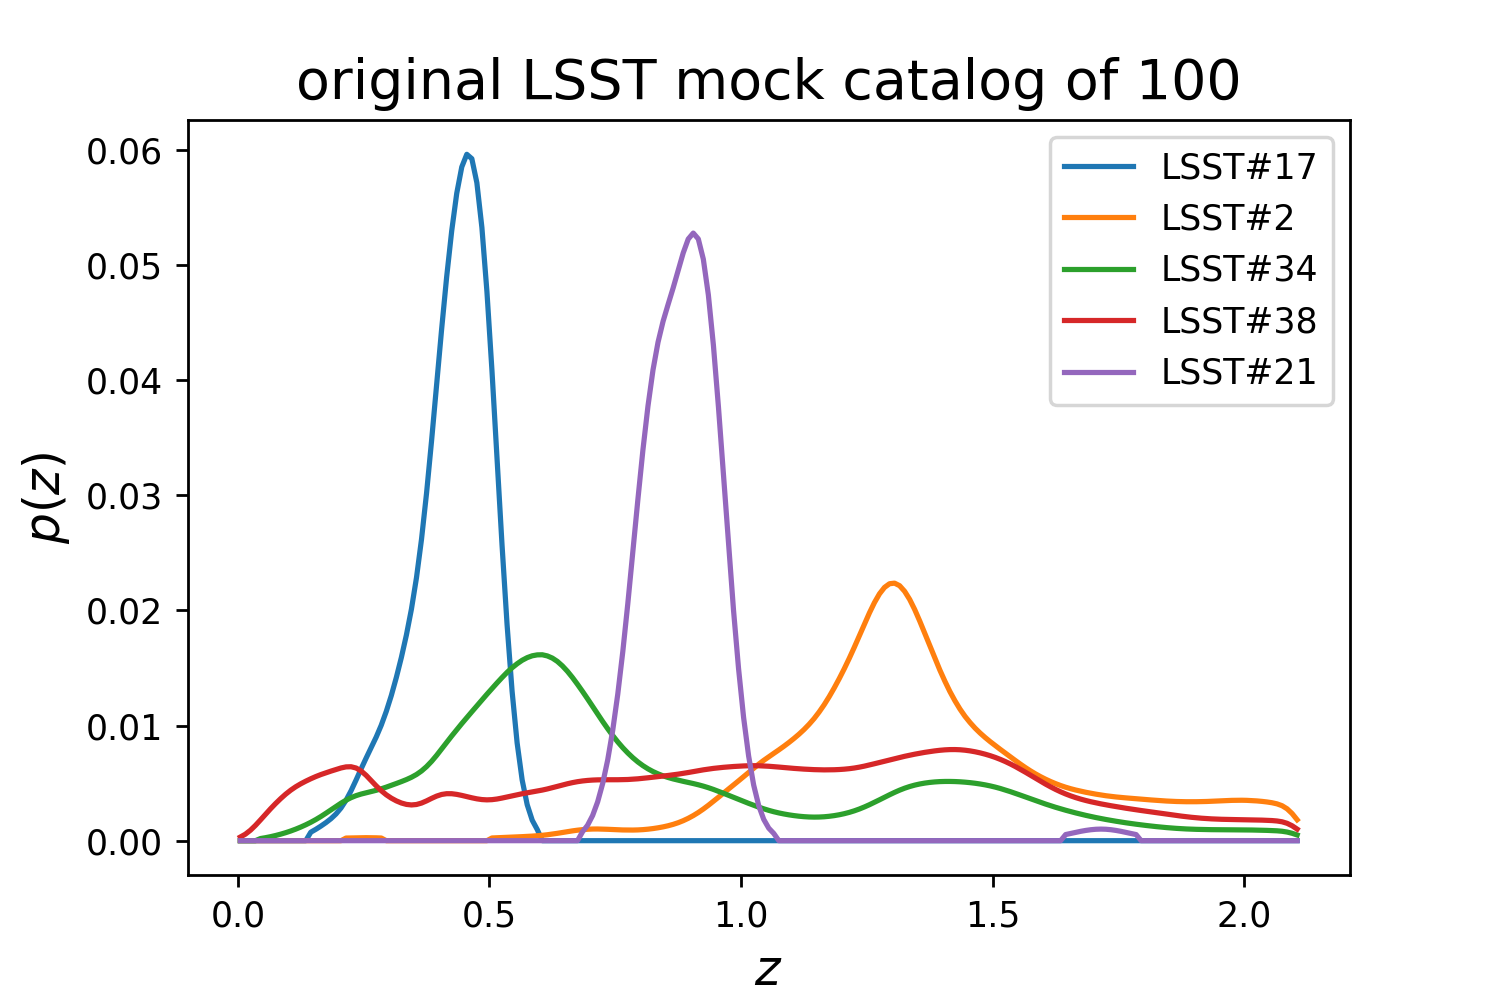
\includegraphics[width=0.9\columnwidth]{figures/lsst_pz_placeholder.png}\\
  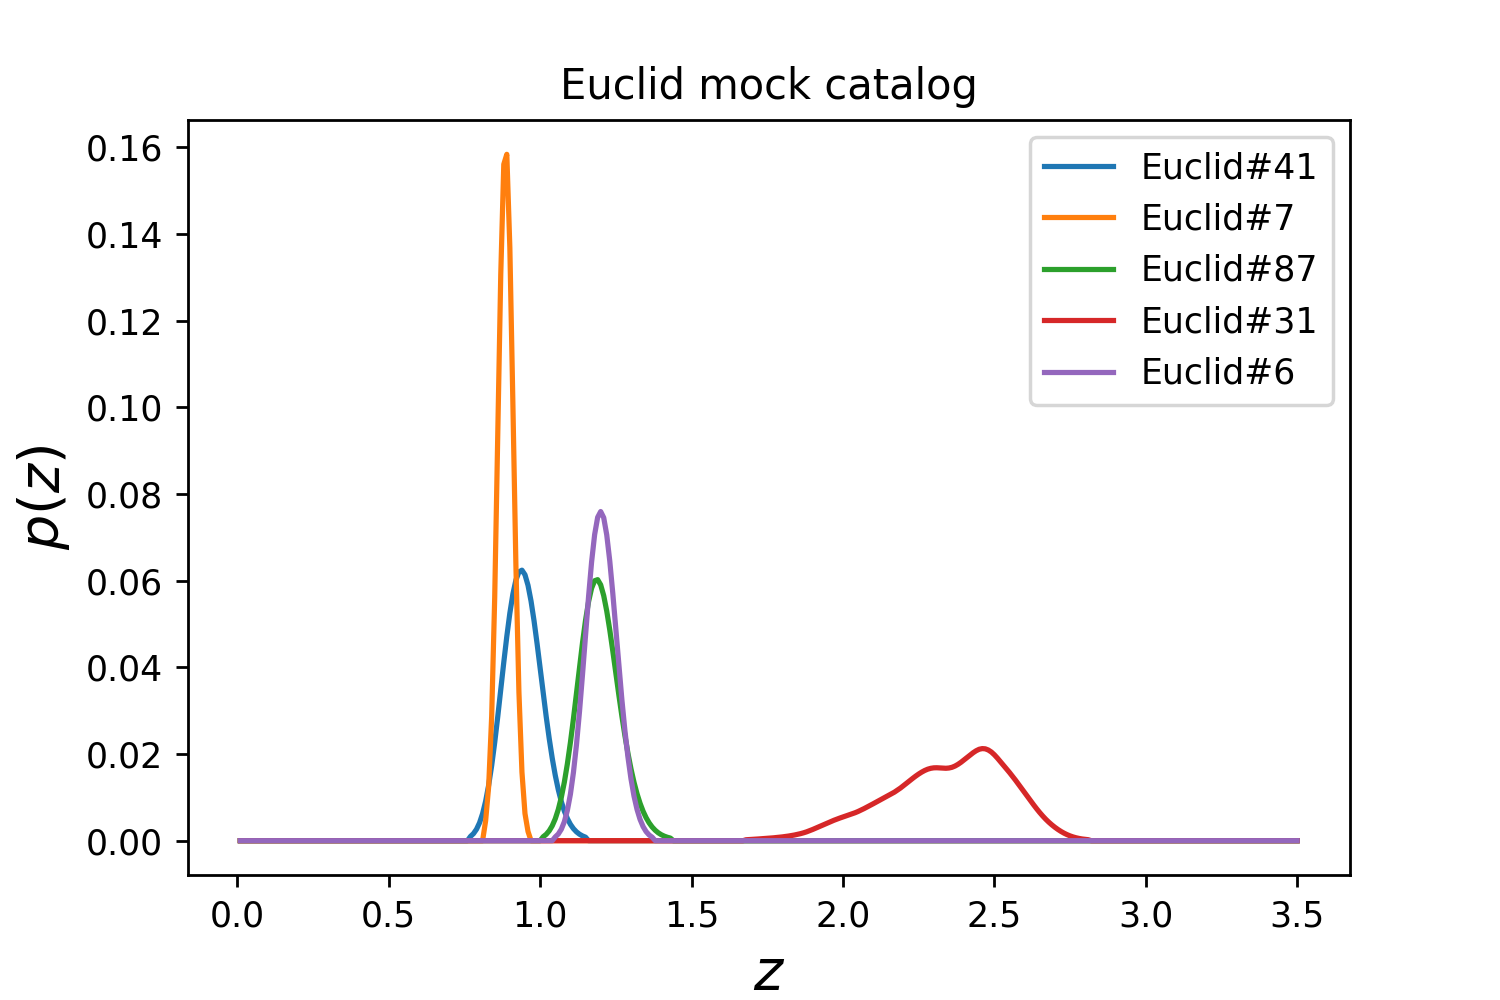
\includegraphics[width=0.9\columnwidth]{figures/euclid_pz_placeholder.png}
  \caption{The shapes of the \pz s\ in the two datasets considered vary 
substantially despite using the same \pz\ method, due to the differences in the 
quality of the photometry.  Different parametrizations may perform better on 
some \pz\ shapes than others.  Top panel: The lower quality photometry of the 
ground-based optical photometry catalog yields broader, multimodal \pz s. 
Bottom panel: The higher quality photometry of the space-based optical + IR 
photometry catalog yields narrow, unimodal \pz s.
  \label{fig:pzs}}
\end{figure}

\subsection{Ground-based optical mock data}
\label{sec:LSST}


In order to simulate the expected LSST galaxy sample, we use the 
Buzzard-highres-v1.0 mock galaxy catalog
, which adds galaxies with SEDs drawn from an empirical library of 
$\sim500,000$ SEDs from the Sloan Digital Sky Survey  (SDSS)
Given an SED, redshift, and absolute r-band magnitude for each galaxy, we 
compute the expected apparent magnitudes and magnitude errors in the six 
broadband LSST filters (ugrizy), assuming full 10-year depth of the survey 
using the simple model of \citet{ivezic_lsst:_2008}.  The catalog contains 
111,171 galaxies to a depth of $i<26.9$, 1.5 magnitudes deeper than the 
expected "LSST Gold sample'' of galaxies that will have S/N$\gtrsim$30 in 
multiple bands.

In implementing BPZ, we create a custom Bayesian prior using a subset of the 
Buzzard-highres-v1.0 catalog, and create a spanning template set via a simple 
k-means clustering algorithm, selection 100 of the SDSS SEDs used in creating 
the Buzzard catalog.  BPZ outputs the marginalized redshift posterior on a 
regular grid of test redshifts, in this case we have 211 points spanning 
$0.005\leq z\leq2.105$.

Even with six filters spanning the optical, there are known degeneracies 
(e.~g.~the Lyman/Balmer break degeneracy) that lead us to expect the presence 
of multi-modal \pz's; some examples are shown in the top panel of 
Fig.~\ref{fig:pzs}.  We produce "true" underlying \pz s by fitting a 
five-component Gaussian mixture model to each \pz\ output by BPZ.


\subsection{Space-based optical + IR mock data}
\label{sec:Euclid}


We start with a 30,000 object subset of the same simulated galaxy catalog used 
for LSST photometric redshift experiments by Graham, et al. (in prep.), which 
is based on the Millennium simulation \citep{springel_simulations_2005}, in 
particular the LC DEEP Gonzalez2014a
catalog based on the galaxy formation models of \cite{gonzalez-perez_how_2014}, 
and was created using the lightcone construction techniques described by 
\cite{merson_lightcone_2013}.  We limit the sample to galaxies with a catalog 
$i$-band magnitude of $i<25$ and true redshifts $z<3.5$. As in Graham, et al. 
(in prep.) we simulate observed apparent magnitudes from the true catalog 
magnitudes by adding a normal random scatter with a standard deviation equal to 
the predicted magnitude error for each galaxy (from Section 3.2.1. of 
\citealt{ivezic_lsst:_2008}, using the software of 
\citealt{connolly_end--end_2014}, assuming a mean airmass of 1.2 and a 10-year 
accumulation of 56, 80, 184, 184, 160, and 160 visits in filters $ugrizy$, 
respectively).  We also ignore any magnitudes fainter than the predicted 
10-year limiting magnitudes in each filter, $u<26.1$, $g<27.4$, $r<27.5$, 
$z<26.1$, and $y<24.9$, as a realistic simulation of non-detections.

The \pz s for this simulated catalog use the CFHTLS set of spectra 
\citep{ilbert_accurate_2006} and all of the default parameter settings for BPZ, 
except that we impose a maximum photometric redshift of 3.5 and allow BPZ to 
use the $i$-band as a magnitude prior during the photo-$z$ fit. The \pz s from 
BPZ are in the form of $N_{ff} = 351$ floating point numbers represing the 
probability on a regular grid of redshifts $0.01 < z_{\rm phot} < 3.51$.  We 
produce "true" underlying \pz s by fitting a three-component Gaussian mixture 
model to each \pz output by BPZ.



\section{Results \& Discussion}
\label{sec:results}


In this study, we perform tests comparing the parametrizations of Sec. 
\ref{sec:approx} as a function of the number of parameters per galaxy.  The 
tests are conducted using the functionality of the \texttt{qp.Ensemble} class 
that is a wrapper for collections of \texttt{qp.PDF} objects.

\subsection{Individual \pz s}
\label{sec:individual}

Parametrizations are compared on the basis of the distributions of the KLD of 
Sec. \ref{sec:metric} calculated over all \pz s in the ensemble.  An example of 
the distribution of the KLD for $N_{f}=10$ is shown in Fig. 
\ref{fig:individual}.

\begin{figure}
  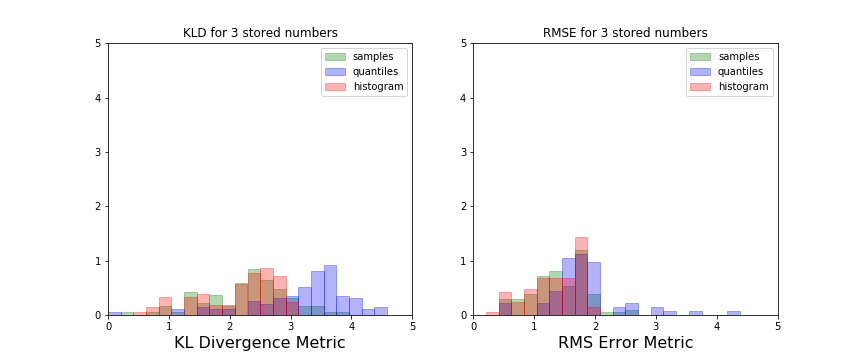
\includegraphics[width=0.9\columnwidth]{figures/individual_placeholder.png}
  \caption{Here one can see the general shape of the distribution of log-KLD 
values for one dataset and one number of parameters over different formats 
(quantiles in purple, samples in green, and histogram in orange).  We note 
that\dots is broad/narrow but high/low\dots.
  \label{fig:individual}}
\end{figure}

To distill what is observed in plots like Fig. \ref{fig:individual} for both 
datasets and all numbers of parameters, we compare the moments of the 
distributions of metric values for the individual \pz s under each 
parametrization, summarized in Fig. \ref{fig:moments}.

\begin{figure}
  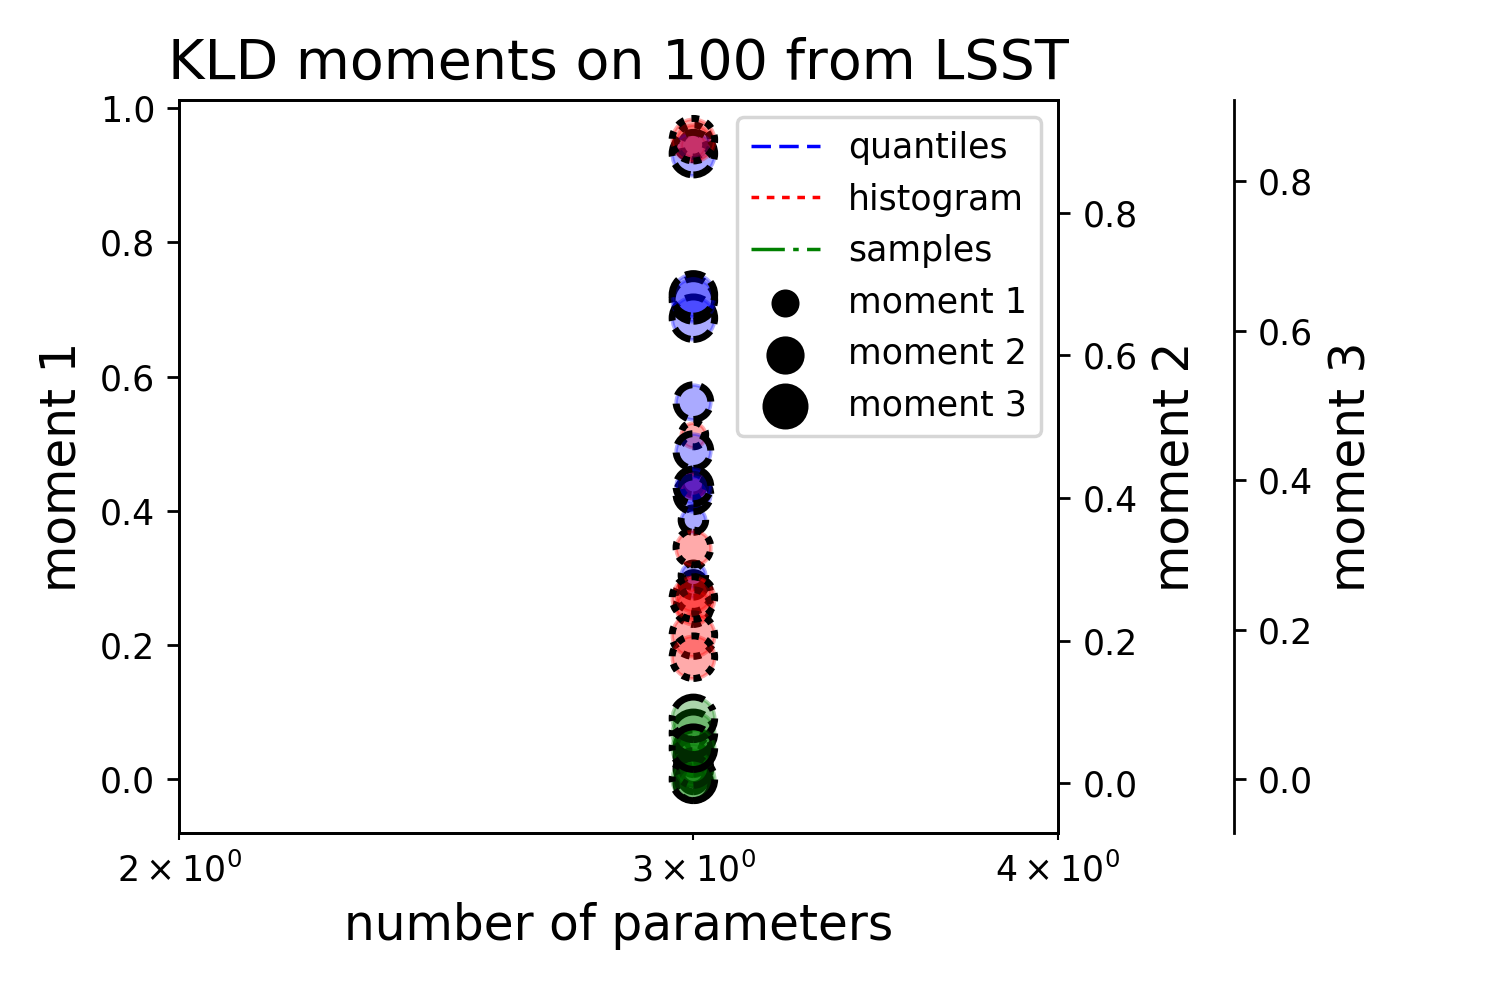
\includegraphics[width=0.9\columnwidth]{lsst_moments_placeholder.png}\\
  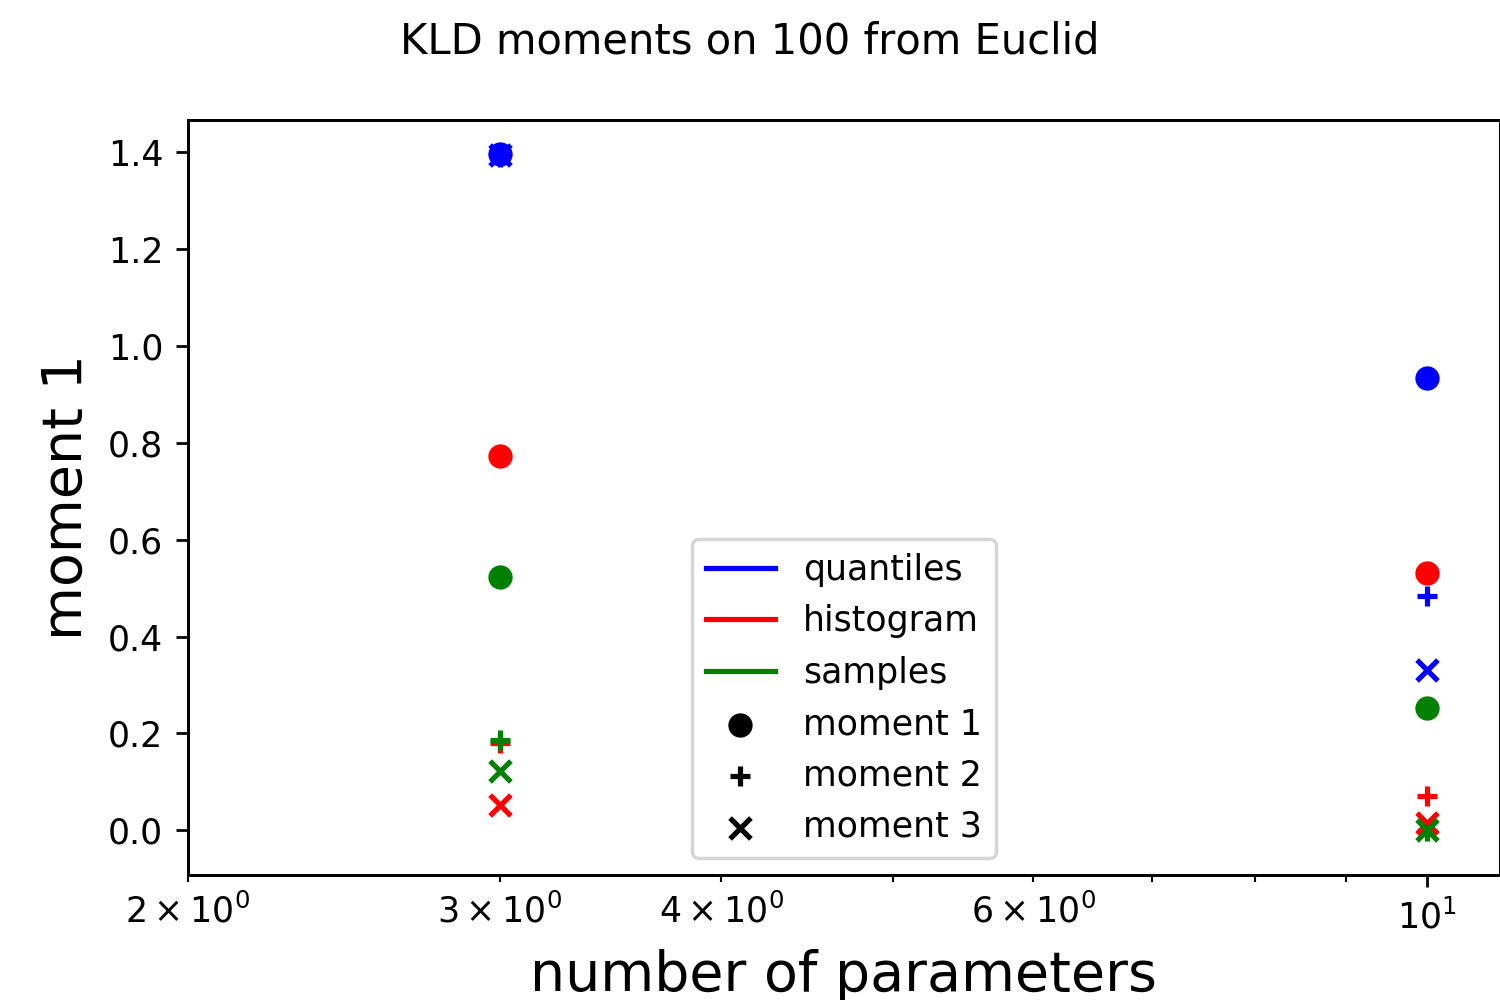
\includegraphics[width=0.9\columnwidth]{euclid_moments_placeholder.png}
  \caption{The mean (star), variance ($\plus$), and kurtosis ($\times$) of the 
KLD distributions are plotted for each dataset over all parametrizations 
(quantiles in purple, samples in green, and histogram in orange).  Top panel: 
The optical dataset has\dots.  Bottom panel: The optical+IR dataset has\dots.
  \label{fig:moments}}
\end{figure}

While it is obvious that one would like the mean (first moment) of the KLD 
distribution to be low, interpretation of higher-order moments is less clear.  
In a science application that is robust to \pz\ outliers, a parametrization 
with a high variance (second moment) may be acceptable, whereas in another 
science application that simply requires well-characterized errors could 
tolerate a higher mean in exchange for a lower variance.  To meaningfully 
interpret the KLD of individual \pz s, it will be necessary for those using \pz 
s in their science to calculate the requirements on the acceptable degree of 
information loss.

\subsection{Stacked $\hat{n}(z)$ estimator}
\label{sec:stacked}

Parametrizations are also compared by the accuracy of their stacked redshift 
distribution estimator $\hat{n}(z)$ relative to that of the \pz s in their 
original format.  Fig. \ref{fig:stacked} shows a typical example of the stacked 
estimator based on \pz s reconstructed from a set number of stored parameters 
under each format, as well as the KLD for each format.

\begin{figure}
  
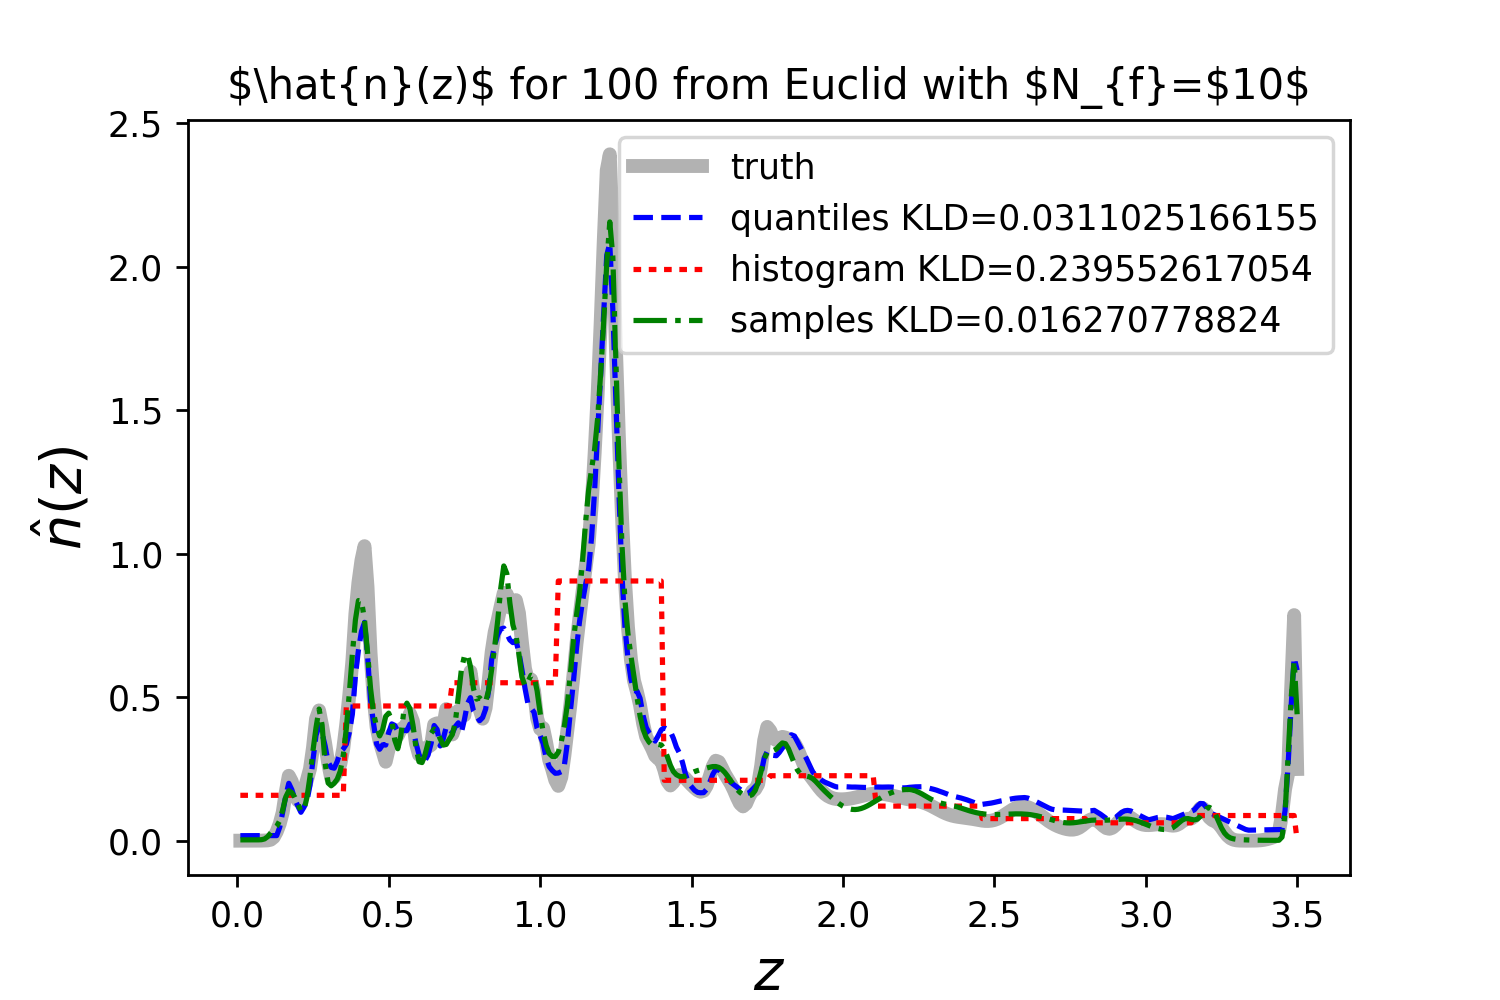
\includegraphics[width=0.9\columnwidth]{figures/euclid_stacked_placeholder.png}
  \caption{We show an example of the stacked estimator of the redshift 
distribution for one dataset with one number of parameters across all formats 
along with the KLD for each format.  The most striking characteristic of 
$\hat{n}$ with a relatively small number of parameters $N_{f}=10$ is the 
coarseness of the histogram format (orange dotted line) relative to the 
quantile format (purple dashed line) and samples format (green dash-dotted 
line), both of which are fairly close to $\hat{n}(z)$ derived from evaluating 
the true \pz s (thick gray line).
  \label{fig:stacked}}
\end{figure}

The KLD values based on plots like Fig. \ref{fig:stacked} over all 
parametrizations are collected and plotted in Fig. \ref{fig:kld}.  Error 
regions are based on $10$ subsamples of $N_{g}=1000$ \pz s from the full 
catalogs of Sec. \ref{sec:data}.  The results can be interpreted in terms of 
absolute accuracy of the redshift distribution estimator and its convergence 
behavior.

\begin{figure}
  
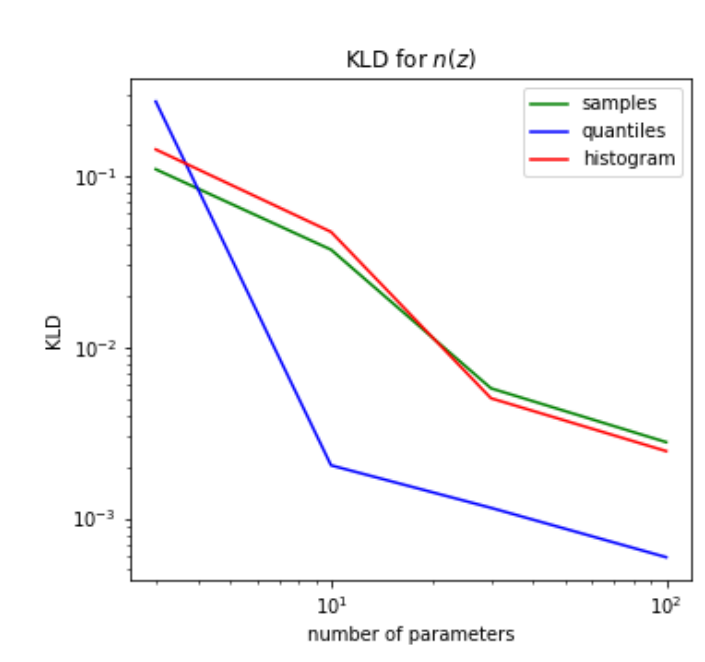
\includegraphics[width=0.9\columnwidth]{figures/lsst_stacked_placeholder.png}\\
  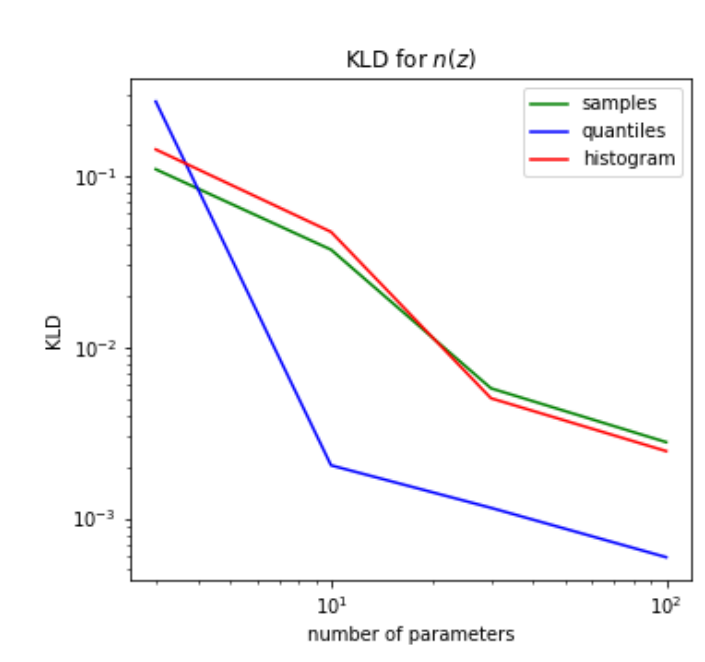
\includegraphics[width=0.9\columnwidth]{figures/lsst_stacked_placeholder.png}
  \caption{We show the behavior of the KLD as a function of number of 
parameters over the quantiles (purple dashed line), samples (green dash-dotted 
line), and histogram (orange dotted line) formats.  Top panel: The Optical 
dataset of Sec. \ref{sec:LSST} shows\dots.  Bottom panel: The Optical+IR 
dataset of Sec. \ref{sec:Euclid} shows\dots.
  \label{fig:kld}}
\end{figure}

A survey may be limited by a required accuracy on $\hat{n}(z)$ for its primary 
science mission or by a hard limit on the available storage $N_{f}$ (or both).  
If the storage is the strongest constraint, one may consider a vertical line in 
Fig. \ref{fig:kld}; the best parametrization will correspond to the format that 
minimizes the KLD at the limiting value of $N_{f}$.

Further recommendations can be made if the requirements on the science products 
derived from the \pz\ catalog are known in terms of the acceptable degree of 
information loss.  If the information loss tolerance on $n(z)$ for a given 
survey mission is specified, it would correspond to a horizontal line in Fig. 
\ref{fig:stacked}; the optimal format would be the one that drops below that 
line at the lowest value of $N_{f}$, which would be the optimal number of 
parameters to store.  We encourage the community to specify the requirements on 
estimators of science products like $n(z)$ in terms of information theoretic 
quantities such as entropy, as these are naturally relatable to \pz s.

If there is some flexibility in the acceptable degree of information loss on 
$\hat{n}(z)$ and/or the allocation of storage for \pz s, as is the case for 
LSST, it may be best to examine the asymptotic behavior of the KLD as a 
function of $N_{f}$ for each format considered to make a choice based on a 
marginal difference.  For example, if the KLD can be significantly reduced with 
a slightly larger $N_{f}$, it may be possible to request additional storage 
capacity for the survey's \pz s.  We note that for these datasets, the KLD 
achieves its asymptote at different values of $N_{f}$ for each format, with the 
histogram format taking far larger $N_{f}$ than the other formats.





\section{Conclusions \& Future Directions}
\label{sec:conclusions}


This work develops a principled approach to choosing a storage format and 
resolution for storing a catalog of \pz s from a survey of known data quality 
to balance the accuracy of \pz s and science products thereof reconstructed 
from the stored parameters against the available storage constraints.  We 
demonstrate the recommended method on two realistic mock datasets 
representative of upcoming \pz\ catalogs and draw the following conclusions:
\begin{itemize}
  \item
  \item As indicated by the KLD, the quantile parametrization is a promising 
option for minimizing loss of information in \pz\ storage.
  \item Given the constraint that LSST will be able to store 200 floating point 
numbers to quantify the redshift of each galaxy and intends to include several 
\pz\ codes, we can safely say that LSST can store the output of more than one 
\pz\ code without any significant risk of loss of information.
\end{itemize}

We also make publicly available the \qp\ Python package central to this 
procedure and invite the community to contribute additional formats and metrics 
to the project.  \qp\ is a tool that can be used to optimize the choice of 
stored parametrization and number of stored parameters of a catalog of \pz s 
based on the accuracy needs of the use cases of the catalog.  Further 
applications of \qp\ functionality for manipulations of \pz s is demonstrated 
in the LSST-DESC PZ DC1 paper (in prep.).

We do not advocate for a one-size-fits-all solution to the problem and 
emphasize that the optimal choice must depend on the requirements of the 
science metric(s) and characteristics of the underlying \pz\ catalog.  
Furthermore, this procedure does not address the computational resources that 
may be necessary to perform the storage operation and to reconstruct \pz s into 
the format necessary for science calculations.

\dots


\subsection*{Appendix}
\label{sec:kld}


\subsection*{Acknowledgments}


SJS was partially supported by the National Science Foundation under grant 
N56981CC


%
%This is the text imported from \code{acknowledgments.tex}, and will be replaced by some standard LSST DESC boilerplate at some point.
%


Author contributions are listed below. \\
A.I.~Malz: Initiated project, led development work. \\
P.J.~Marshall: Advised on statistics, and project design and management. \\
S.J.~Schmidt: Produced the PDFs for the fainter mock catalog. \\
M.L.~Graham: Produced the photometry and PDFs for the brighter mock catalog. \\
J.~DeRose: Produced the photometry for the fainter mock catalog. \\
R.~Wechsler: Supervised production of the fainter mock catalog. \\



\bibliography{lsstdesc,main}

\end{document}
